\section{Results}

The total U.S. Resource is estimated to be between 3255 and 3920 TWh/yr (Table~\ref{table:totals}). Roughly half of this is contained in the remote resource, and the other half is due to the local resource. Roughly 2/3 of this resource is in Alaska where a large resource area and energetic waves in the North Pacific combine to create a large total. The U.S. West Coast has a large remote resource where energetic waves from the North Pacific arrive from offshore.  The West Coast remote resource is, relatively, modest. The U.S. East Coast resource, on the other hand, is composed primarily of the local resource and has a relatively modest remote portion. This is because mid-latitude westerly winds tend to generate wave energy that propagates eastward, and relatively less wave energy from the open ocean propagates onshore from the open ocean (compared to the West Coast). This also indicates that much of the East Coast wave resource is located farther from shore, where there is sufficient fetch to have created energetic waves. \note{Is that last sentence accurate? Assuming yes, is a citation needed for that or is it `simple physics'-enough to simply be stated?}

Hawaii has a large resource due largely to waves that arrive from the North Pacific along the northern boundary of the EEZ surrounding the islands. The local resource is relatively small, due primarily to the fact that the sea-state in this region is -- in the long-average perspective presented here, and compared to regions such as the East Coast where wave growth dominates -- roughly `steady-state' because the wind input and dissipation are relatively balanced. The Caribbean region (Gulf of Mexico, Puerto Rico, and U.S. Virgin Islands) on the other hand, has a modest wave resource composed predominantly of local wind input. \note{Is ``the Caribbean region'' a term, or is there something better I should use?} The remote resource of this region is also very small because the majority of the U.S. EEZ boundary throughout this region borders other EEZs (rather than being exposed to the open ocean), and the methodology described here only counts wave energy crossing into the EEZ from the open-ocean. \note{Do we need to add an average wave-flux to the tables (kW/m)?}

\begin{table}[ht]
  \centering
  \begin{tabular}{|c|c|c|c|c|}
    \hline
    %\multirow{2}{*}{Region}
    Region & Remote & \multicolumn{2}{c}{Local} & Total \\
    & & Natural & Potential & \\
    \hline
    Alaska & 1040 & 960 & 1390 & 2000 - 2430 \\
    West Coast & 420 & 90 & 190 & 510 - 610 \\
    Hawaii & 370 & 10 & 90 & 380 - 460 \\
    East Coast & 110 & 170 & 210 & 280 - 320 \\
    Gulf of Mexico & 13 & 50 & 60 & 63-73 \\
    P.R. \& U.S.V.I. & 6 & 11 & 26 & 17 - 32 \\
    \hline \hline
U.S. TOTAL & 1959 & 1296 & 1961 & 3255 - 3920 \\
\hline
  \end{tabular}
  \caption{Wave resource assessment results by region and totaled for the entire U.S. (all values in TWh/yr). The range in the total column indicates the sum of Remote+Local (lower value) and Remote+Potential (higher value). \note{We need to confirm these values again.}}
  \label{table:totals}
\end{table}

\begin{figure}[ht]
  \centering
  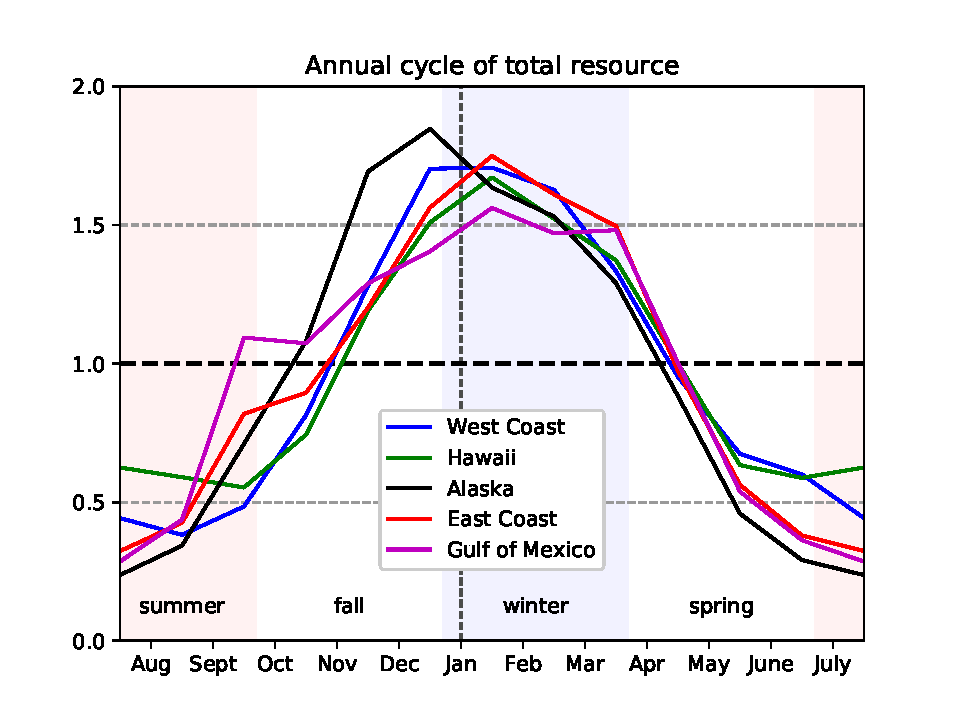
\includegraphics[width=\textwidth]{../fig/AnnualCycle01.pdf}
  \caption[Wave resource annual cycle.]{The annual cycle of the total wave energy resource for several regions, relative to the regional mean.}
  \label{fig:annual-cycle}
\end{figure}


\begin{figure}[ht]
  \centering
  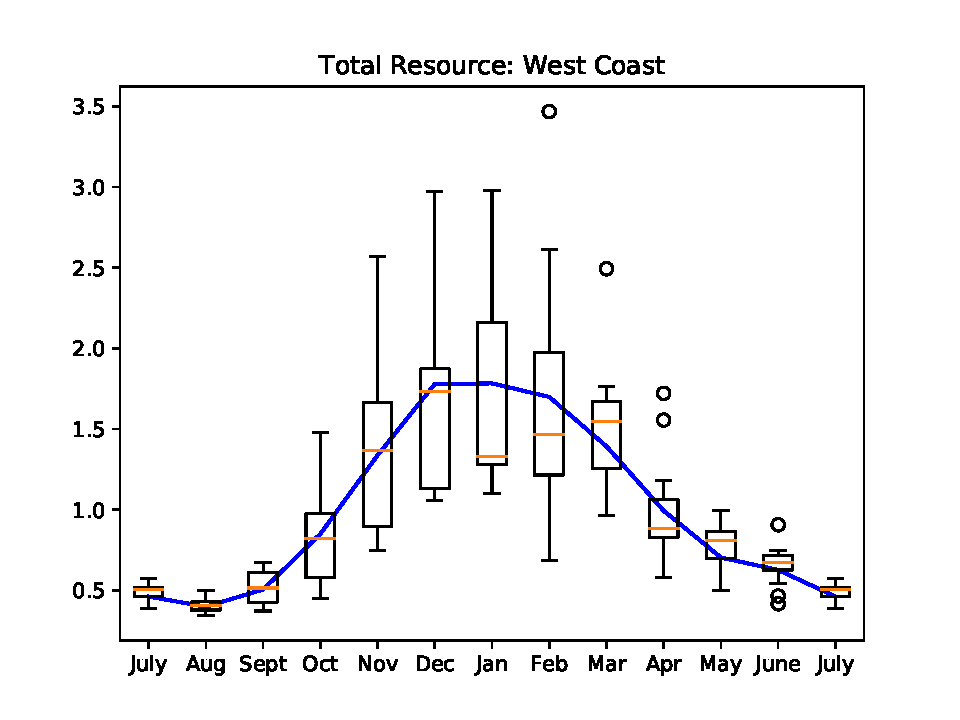
\includegraphics[width=\textwidth]{../fig/AnnualVar01.wc.pdf}
  \caption[West Coast resource variability.]{Annual and inter-annual variability of the West Coast resource. The thick solid line indicates the mean, and the orange lines and boxes indicate the median and quartiles, respectively. The whiskers extend to the last point within 1.5x of the inter-quartile range, and points beyond this are plotted as open-circles.}
  \label{fig:wc-variability}
\end{figure}

The annual cycle of the wave energy resource has a remarkably consistent pattern across all U.S. regions (Figure \ref{fig:annual-cycle}). Wave energy is a late-fall and winter dominated resource. The resource peaks in December or January across all regions, and is at a minimum in summer months. The inter-annual variability of the monthly-averaged West Coast resource is small during summer months when the resource is small (Figure \ref{fig:wc-variability}). During energetic winter months, the monthly-averaged resource can vary by more than 50\%, but in general the interannual variability is less than 30\% of the month's mean. This suggests that during energetic winter months wave energy projects should be expected to deliver at least their annual mean, with the potential of providing up to three-times that value. \note{Is that last sentence a stretch? Am I glossing over too many details about site-specific variability and device performance characteristics?} However, more detailed analysis is required to demonstrate these characteristics at individual sites and for individual technologies. Other regions have similar variability characteristics (not shown for simplicity).

The large increase in resource in Hawaii is due in large part due to the exteneded area of integration. In the EPRI 2011 report the integration was performed at the 200 m isobath, which in the case of Hawaii is very close to shore due to the lack of continental shelf. In the present case, integration contour is extented to the EEZ which lies at 200 nmi in the Northern, Eastern, and Southern boundaries.

\begin{table}[ht]
  \centering
  \begin{tabular}{|c|c|c|c|}
    \hline
    Region 
    &
      \begin{tabular}{c}
        EPRI 2011 \\ {\it Remote Only} \\ $\mathrm{[TWh/yr]}$
      \end{tabular}
    &
      \begin{tabular}{c}
        New Total \\ TWh/yr
      \end{tabular}
    & \% Change \\
    \hline
    West Coast & 590 & 510 - 610 & -5 $\pm$10 \\
    Hawaii & 130 & 300 - 380 & +160 $\pm$30 \\
    East Coast & 240 & 280 - 320 & 25 $\pm$8 \\
    Gulf of Mexico & 80 & 63 - 73 & -15 $\pm$7 \\
    Alaska & 1570 & 2000 - 2430 & +40 $\pm$15 \\
    P.R. \& U.S.V.I. & 30 & 17 - 32 & -20 $\pm$25 \\
    \hline \hline
    U.S. TOTAL  & 2640 & 3170 - 3845 & +33 $\pm$ 13 \\
    \hline
  \end{tabular}
  \caption{Wave resource totals compared to 2011 results (all values in TWh/yr).}
  \label{tab:total-compare}
\end{table}

\begin{figure}[ht]
  \centering
  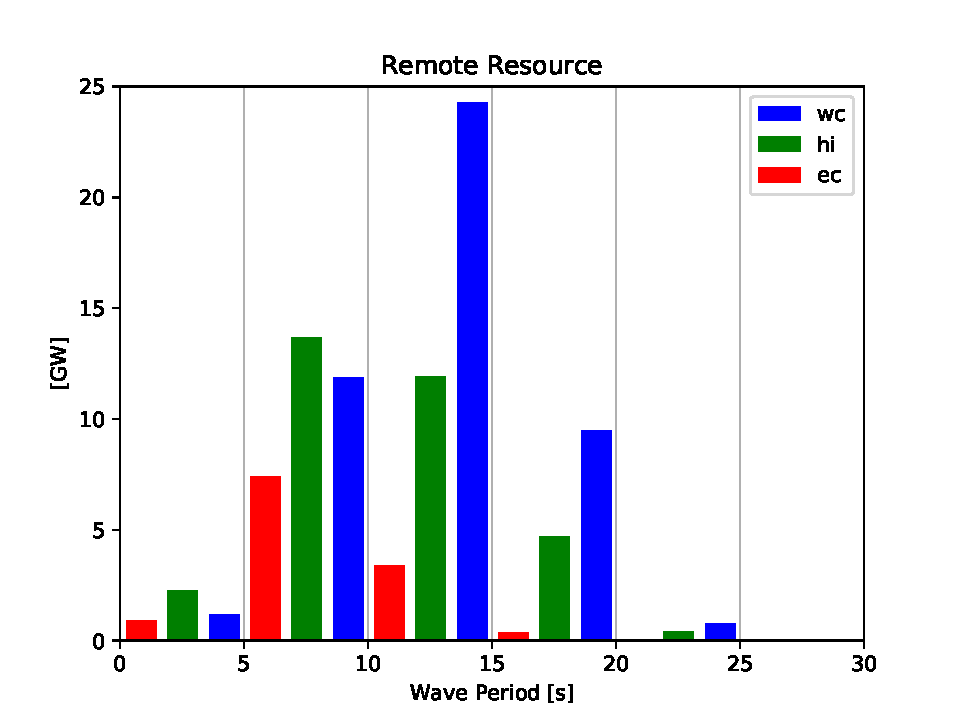
\includegraphics[width=\linewidth]{../fig/RemoteResource_Freq01.pdf}
  \caption{Remote resource contained in each wave period band (0-5 seconds, 5-10 seconds, etc.) for the west coast, Hawaii, and the east coast.}
  \label{fig:remote-freq}
\end{figure}

\begin{figure}[ht]
  \centering
  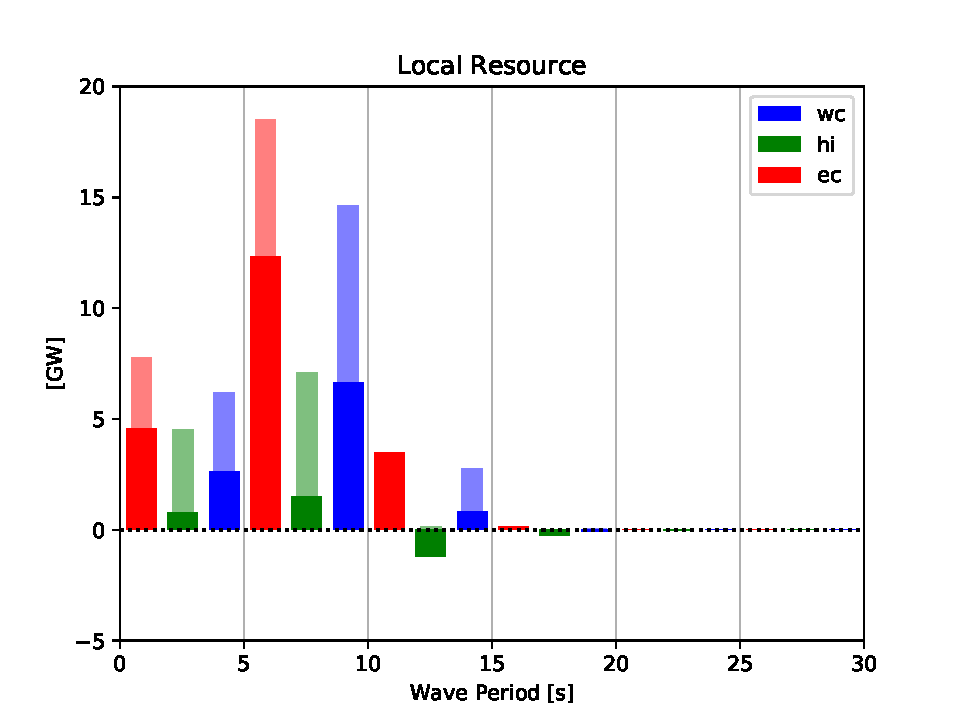
\includegraphics[width=\linewidth]{../fig/LocalResource_Freq01.pdf}
  \caption{Local (thick solid bars) and potential (narrow pale bars) resource contained in each wave period band (0-5 seconds, 5-10 seconds, etc.) for the west coast (wc), Hawaii (hi), and the east coast (ec).}
  \label{fig:remote-freq}
\end{figure}

\begin{itemize}
\item Plots of ‘remote’ resource vs. distance from shore (Figure 5). ... How does this compare with local resource vs. distance from shore?
\item Remote resource vs. depth. Local resource vs. depth.
\end{itemize}


%%% Local Variables:
%%% TeX-master: "wave_res"
%%% End:
